%----------------------------------------------------------------------------------------
%	PACKAGES AND OTHER DOCUMENT CONFIGURATIONS
%----------------------------------------------------------------------------------------


\documentclass[12pt,oneside,final,a4paper]{report}
\usepackage{generators/imports}

%\makeglossaries      % alt 1
\makenoidxglossaries  % alt 2

\renewcommand*{\acronymname}{List of Acronyms and Abbreviations}
\renewcommand{\glsnamefont}[1]{\textbf{#1}}

%Create acronyms here.
\newacronym{saas}{SaaS}{Software as a Service}
\newacronym{vcs}{VCS}{Version Control System}
\newacronym{CNN}{CNN}{Convolutional Nural Network}
\newacronym{FCNN}{FCNN}{Fully Connected Nural Network}

%You can also do explanations.
\newglossaryentry{git}{name={Git},
    description={Git is a \gls{vcs} for tracking changes in computer files and coordinating work on those files among multiple people}}
\newglossaryentry{ai-model}{name={\ensuremath{\Theta_{AI}}},
    description={AI-model is the \gls{CNN} or \gls{FCNN} we want to teach to a human.}}

\begin{document}
\begin{titlepage}

\newcommand{\HRule}{\rule{\linewidth}{0.5mm}} % Defines a new command for the horizontal lines, change thickness here

\center % Center everything on the page
 
%----------------------------------------------------------------------------------------
%	HEADING SECTIONS
%----------------------------------------------------------------------------------------

\textsc{\LARGE University of Bergen \\ Department of Informatics}\\[1.5cm] % Name of your university/college

%----------------------------------------------------------------------------------------
%	TITLE SECTION
%----------------------------------------------------------------------------------------

\HRule \\[0.5cm]
\begin{Huge}
	\bfseries{Machine Teaching using minimzation over complexity of instances}\\[0.7cm] % Title of your document
\end{Huge}
\HRule \\[0.5cm]

%----------------------------------------------------------------------------------------
%	AUTHOR SECTION
%----------------------------------------------------------------------------------------

\large \emph{Author:} Brigt Arve Toppe Håvardstun\\
\large \emph{Supervisors:} Jan Arne Telle\\[2cm]

%----------------------------------------------------------------------------------------
%   LOGO SECTION
% 	This will require the graphicx package
%	Change the line to comment if you only want the UiB Logo
%	Logo for other faculties here: http://kapd.h.uib.no/profilmanual/99LastNed/99a_lastned.html
%----------------------------------------------------------------------------------------

\centerline{
\includegraphics[scale=1.9]{figures/canvasWithFaculty}}
%\centerline{
\includegraphics[scale=0.15]{figures/canvas}}  %change for your faculty

%----------------------------------------------------------------------------------------
%	DATE SECTION
%----------------------------------------------------------------------------------------

{\large \monthyeardate\today}\\[3cm] % Date, change the \today to a set date if you want to be precise

%----------------------------------------------------------------------------------------
%	LOGO SECTION
%----------------------------------------------------------------------------------------

\vfill % Fill the rest of the page with whitespace

\end{titlepage}
 % This is the titlepage
\pagenumbering{roman}

\begin{abstract} 

\noindent 
In todays society AI and machine learning is becoming more and more relevant. (find source) For instance, some might say the age old problem of the
protein folding has finally been solved thanks to Deep mind and their Alphafold 2 \cite{jumper_highly_2021} . Their deep learning approach achieved close to 90\% accuray,
matching experimental approaches. However, even if we now can get greatly accurat approximation solutions to the question of protein folding, the question of
how each protein fold into their 3D structure has not been solved yet. Motivated by this fact; that knowing solutions to instances not nessecery gives insight 
to the question at large, as well as the expanding use of AI in our everday life [image recognition, recommendation systems, personal medecin and law]. This places Explaineable AI as a topic of
of extrem relevancy in the comming years. 
Our work will regard the topic of model-agnoitic, global, example baed Explaineable Machine 
Learning. We will focus on the complexity of each instance to be used for teaching, and not on how many examples we are going to use.



\end{abstract}

\renewcommand{\abstractname}{Acknowledgements}
\begin{abstract}
	Est suavitate gubergren referrentur an, ex mea dolor eloquentiam, novum ludus suscipit in nec. Ea mea essent prompta constituam, has ut novum prodesset vulputate. Ad noster electram pri, nec sint accusamus dissentias at. Est ad laoreet fierent invidunt, ut per assueverit conclusionemque. An electram efficiendi mea.
	
	\vspace{1cm}
	\hspace*{\fill}\texttt{Brigt Arve Toppe Håvardtu}\\ 
	\hspace*{\fill}\today
\end{abstract}
\setcounter{page}{1}
\newpage
{
\tableofcontents 
\let\cleardoublepage\clearpage \listoffigures 
\let\cleardoublepage\clearpage \listoftables 
\let\cleardoublepage\clearpage \lstlistoflistings
}
\pagenumbering{arabic}
\setcounter{page}{1}
\setlength{\parskip}{0.5cm plus4mm minus3mm}  

\chapter{Introduction}

In this master thesis we implement and discuss the reulst of the propsed model 
for machine teaching. \cite{CNN:deeplearning}

\section{Background}

Lorem ipsum dolor sit amet, cu graecis propriae sea. Eam feugiat docendi an, ei scripta blandit pri. Nonumes delicata reprimique nam ut. Eu suas alterum concludaturque est, ferri mucius sensibus id sed~\cite{raftAlg}.

We can do glossary for acronymes and abriviations also: \gls{saas}. As you see the first time it is used, the full version is used, but the second time we use \gls{saas} the short form is used. It is also a link to the lookup.


\subsection{Listings}
You can do listings, like in Listing~\ref{ListingReference}
\begin{lstlisting}[caption={[Short caption]Look at this cool listing. Find the rest in Appendix~\ref{Listing}},label=ListingReference]
$ java -jar myAwesomeCode.jar
\end{lstlisting}

You can also do language highlighting for instance with Golang:
And in line~\ref{LineThatDoesSomething} of Listing~\ref{ListingGolang} you can see that we can ref to lines in listings.

\begin{lstlisting}[caption={Hello world in Golang},label=ListingGolang,escapechar=|]
package main

import "fmt"

func main() {
    fmt.Println("hello world") |\label{LineThatDoesSomething}|
}

\end{lstlisting}

\subsection{Figures}

Example of a centred figure
\begin{figure}[H]
    \centering
    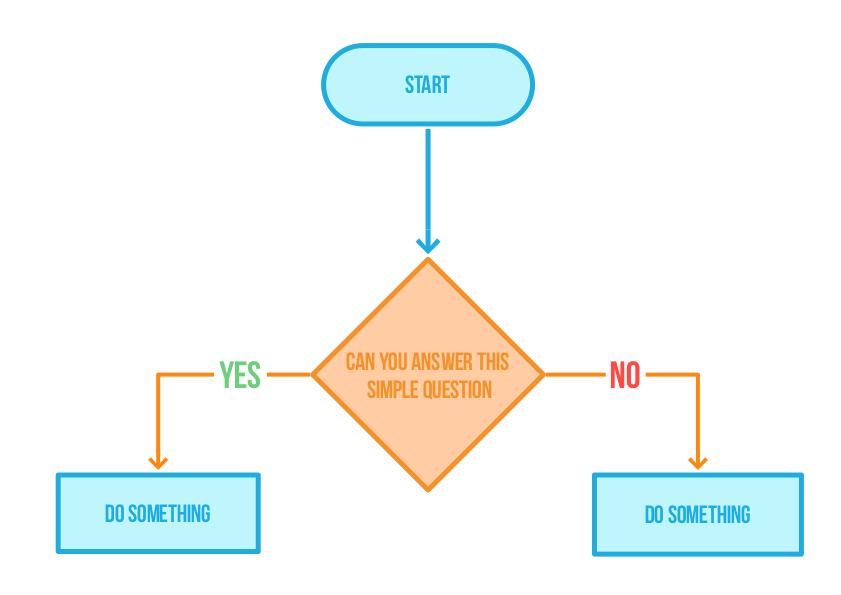
\includegraphics[scale=0.5]{figures/Flowchart}
    \caption{Caption for flowchart}
  	\medskip 
	\hspace*{15pt}\hbox{\scriptsize Credit: Acme company makes everything \url{https://acme.com/}}
    \label{FlowchartFigure}
\end{figure}

\subsection{Tables}

We can also do tables. Protip: use \url{https://www.tablesgenerator.com/} for generating tables.
\begin{table}[H]
\centering
\caption{Caption of table}
\label{TableLabel}
\begin{tabular}{|l|l|l|}
\hline
Title1 & Title2 & Title3 \\ \hline
data1  & data2  & data3  \\ \hline
\end{tabular}
\end{table}

\subsection{\gls{git}}

\gls{git} is fun, use it!
\chapter{Models}

In this thesis there are multiple "models" and we will therefor establish cleare notations and descriptions of 
each.

\section{\gls{ai-model} - the AI model to be learned}

With $\Theta_{ai}$ we refere to the AI model we are trying to teach to a human. 
In this thesis we will experimented with two different implementations of $\theta{ai}$. 
The first being \gls{CNN} \cite{CNN:deeplearning}, and the other being \gls{FCNN}.
$\Theta_{ai}$ will be trained on imags, and will try to preditc a ground truth boolean function. 
This will be discussed in the chapter \nameref{DatasetChap}. Both \gls{CNN} and \gls{FCNN} will be discussed in further implementations detail in [chapter FCNN] and [chapter CNN].

\section{$L_M$ - modeling human learner}
$L_M$ will be an algorithm trying to mimic human behavior. Given a set of \hyperref[InstanceDescription]{instances} and corresponding predicted values, $L_M$ 
outputs a guessed $\Theta_{M}$. \{Should i here discuss different implementations, difficulty of mimicing human behavior etc?\}

\section{$\Theta_{M}$ - $L_M$s model of $\Theta_{AI}$}
$\Theta_{M}$ is the output of $L_M$, and a model of $\Theta_{AI}$. Model is understood as giving the same output on, essentially[note to explaination], the same input.
Our $\Theta_{M}$ will be a boolean function, and hence not take in a bitmap. Rather it takes as input a truth assigment to four literals, 
corresponding to the four litterals "A", "B", "C", and "D". 

\chapter{Dataset}
\label{DatasetChap}

In this chapter we discuss how the dataset was choosen, how we create it, and the different parameters 
acceseable when creating it. 

\section{Background}

Our first decision was in desciding the task our AI was going to solve.
In selecting the task our AI model was going to solve we had a few attributes in mind. We did not want something to complex,
it had to be simple to implement and change,  as we were to make a Proof Of Consept. At the same time the problem should not be too simple,
we want to check if our method will convey the AI models errors with respect to the ground truth.
We also wanted to able to test our system with different AIs. To achive this we wanted our task to achive this we wanted the ground truth
to be easily changeable, so we can compare AIs trained on different ground truths.

In the end we chose the task of predicting an underlaying boolean function given bitmaps contaning a subset of the literals {A,B,C,D}.
Present literals in the bitmap is set to True, and all others are set to False. The label for a given instance is 
then found by calulcateing the underlaying boolean function with literal assigned as descrebied above, giving a label of
1 – being True – or 0 – being False.

This choice fits our demands as we can easily create a new ground truth by swapping the ground truth boolean function. This means our model is not over complex. 
At the same time the bitmaps representation of literals gives us the possibility of huge traing datasets, which has the possibility of creating
more or less complex datasets – different orientations, sizes and letter styles. 

\section{Description of an instance}
\label{InstanceDescription}

In more detail, the input to our AI will be a 64x64 bitmap. The cells in the bitmap will either have the value $0$ or $255$.
The cells having the value $255$ will together make up one or more letter from a predetermined letter set $L = {A,B,C,D}$.
Three examples of the instances are shown below.
 
\begin{figure}[!htb]
    \minipage{0.32\textwidth}
      
\includegraphics[width=\linewidth]{figures/Bitmap-A}
      \caption{Bitmap A}\label{Bitmap-A}
    \endminipage\hfill
    \minipage{0.32\textwidth}
      
\includegraphics[width=\linewidth]{figures/Bitmap-AD}
      \caption{Bitmap AD}
      \label{Bitmap-AD}
    \endminipage\hfill
    \minipage{0.32\textwidth}%
      
\includegraphics[width=\linewidth]{figures/Bitmap-BCD}
      \caption{Bitmap BCD} 
      \label{Bitmap-BCD}
    \endminipage
\end{figure}

% TODO: This seems bad. Maybe fix? Image smaller?
We also have different parameters to active. These will be discussed in \ref{ParametersGenDataset}. 
The images above are of the smallest varience possible. Below are examples showing images 
from our dataset at highest possible varience.

\begin{figure}[!htb]
    \minipage{0.32\textwidth}
      
\includegraphics[width=\linewidth]{figures/Bitmap-highvar-ABCD}
      \caption{Bitmap ABCD}
      \label{Bitmap-highvar-ABCD}
    \endminipage\hfill
    \minipage{0.32\textwidth}
      
\includegraphics[width=\linewidth]{figures/Bitmap-highvar-ABD}
      \caption{Bitmap ABD}
      \label{Bitmap-highvar-ABD}
    \endminipage\hfill
    \minipage{0.32\textwidth}%
      
\includegraphics[width=\linewidth]{figures/Bitmap-highvar-CD}
      \caption{Bitmap CD} 
      \label{Bitmap-highvar-CD}
    \endminipage
\end{figure}


\section{Properties of instance}
We want to have som clear properties for each data instance. These are mostly sanity checks to make sure
our AI will be given decent data. Altough intuitive, its important to make sure our data is sane. 
Bad data in, means bad perdictions comming out. 

Our rules for the data goes as follows:
\begin{itemize}
    \item For each letter, the entirety of the letter is to be contained within the picture. 
    \item No letter is to overlap with another letter. 
    \item The size of the letter should not be to small. The letter shall contain enough pixles, such that the characteristics of the letter is mainteind. E.g. clearly recognizeable for a human.
  \end{itemize}


\section{Parameters generating instances}
\label{ParametersGenDataset}
When generating data we have quite a few differtent parameters, all contributing to more or less complexity
in our data. The goal of having different parameters for dataset generating is to be able to have a smooth increasing 
in difficulty for our AI. Using this we can find a suitable dataset for our AI models, where they preforme resonabley well. 
We can also try to detect different overfittings based on these parameters.

\subsection{$FixedSquares$ – placement of letter}
For the parameter $FixedSquares$ we divide the image into four squares –top left, top right, bottom left, bottom right. 
Each of these square might then contain a letter. Crucially no letter is overlapping these squares.
All of figures \ref{Bitmap-A},  \ref{Bitmap-AD} and \ref{Bitmap-BCD} have $FixedSquares$.
Having this parameter turned on will make the dataset less complex, as its counter part is to just place freely.
Without $FixedSquares$ the algorithm might find all letters at the top of the image or at the bottom, increasing the
varience of the dataset. This corresponds to a more complex dataset, less prone to be easily overfitted.


\subsection{$Rotation$ – orientation of the letter}
With the parameter $Rotation$ we alow the letters to have different orientations. 
We have slected a subset of orientations $O=\{ 0 ^{\circ}, 45^{\circ}, 90^{\circ}, 135^{\circ}, 180^{\circ}, 225^{\circ},270^{\circ},315^{\circ}\}$. 
Letting each letter take on one of these orientations increase varience and complexity in our dataset. 
Below is an example of an image from a dataset with $Rotation$ allowed.
 
\begin{figure}[h]
    \centering
    
\includegraphics[scale=0.2]{figures/Bitmap-rot-ABC}
    \caption{Bitmap w/rotation ABC} 
    \label{Bitmap-rot-ABC}
\end{figure}

\subsection{$Scale$ - size of the letter}
With $Scale$ we allow letters to have different sizes. Importantly no letter can be made to big \ref{Bitmap-big-ACD}, as
it has to fit inside the image. Nor can it be made to small \ref{Bitmap-small-AB}, as it needs to be recognizeable. 

\begin{figure}[!htb]
    \minipage{0.4\textwidth}
      
\includegraphics[width=\linewidth]{figures/Bitmap-big-ACD}
      \caption{Bitmap ACD, too big. Overlapping, and out of image.}
      \label{Bitmap-big-ACD}
    \endminipage\hfill
    \minipage{0.4\textwidth}
      
\includegraphics[width=\linewidth]{figures/Bitmap-small-AB}
      \caption{Bitmap AB, too small. A is broken up, B looks like R.} 
      \label{Bitmap-small-AB}
    \endminipage
\end{figure}

Having a broader range of sizes on the images will increase varience and complexity of our dataset.

\section{Labels}
After having described our data instance, we now describe the corresponding labels in the dataset.
Our labeles will hold either the value $0$ or the value $1$. This corresponds to our ground truth boolean function returing 
True ($1$) or False ($0$). When evalueting a instance we retrive letters used to genereated this instace,
and set the corresponding letters to true in our ground truth boolean function, and letters not present will be set to false.
For instance given ground truth boolean function $(A $ and not $ B)$ \nameref{Bitmap-A} would be true, and hence 
get label $1$, while \nameref{Bitmap-highvar-ABD} would be false and have label $0$

% Include more chapters as required.
%%=========================================

% Alternative 1 of printing glossaries & acronymes
%\renewcommand{\glossarypreamble}{\footnotesize}
%\printglossary[style=super, type=\glsdefaulttype] \let\cleardoublepage\clearpage
%\printglossary[style=super, type=\acronymtype]


%Alternative 2
%Simplified way of printing glossaries, slower than alt 1, but has better compatibility
\printnoidxglossaries

% Include more appendices as required.
%%=========================================
\clearpage
\DeclareRobustCommand{\VAN}[3]{#3}
\addcontentsline{toc}{chapter}{Bibliography}
\bibliographystyle{generators/myplainnat}
\bibliography{generators/refs}
\appendix
\titleformat{\chapter}[display]
  {\normalfont\large\bfseries}% <- font for label "Appendix A", default \huge
  {\chaptertitlename\ \thechapter}
  {20pt}
  {\large}% <- font for title, default \Huge

\chapter{Generated code from Protocol buffers}

\begin{lstlisting}[caption={Source code of something},label=Listing]
System.out.println("Hello Mars");
\end{lstlisting}
\end{document}
